\chapter{Background}
\label{ch:background}

% Explain the background and theory underlying your project.
% Assume that the average reader has the same knowledge you had \emph{before} undergoing this project.
% This chapter should transfer all knowledge necessary to understand the following chapters.

% As this and the following chapters are likely longer than a few pages, consider structuring them into sections (but avoid fragmentation by overly fine-grained sectioning).
% Use the \verb|\..section{}| command family as illustrated below:

Before we look into the algorithms and theory behind reordering techniques, we first take a dive into the factorization process that produces further non-zeroes, which in this and the entire thesis's context, are called fill-in. It may be trivial but important to note, that if some numerical arithmetic results in a zero in the factored matrix, it is usually still considered as a fill-in. 

Suppose the set of set of \textit{n} equations that are to be solved are
\begin{equation}
    Ax = b
\end{equation}
where \(A\) is a sparse matrix, \(x\) is the vector of unknowns. The sparsity, or the number of non-zero entries in \(A\) determines the fill-in of it's Cholesky factor when it is employed to solve the aforementioned set of equations. 
Suppose the Cholesky factorization of \(A\) is given by \(LL^T\), where \(L\) is a lower triangular matrix (with a positive diagonal) and \(L^T\) is the transpose of \(L\). The efficiency of solving this set of equations is dependent on the number of non-zero entries in \(L\). It has been shown that we can factor and solve the set of equations in space proportional to  \(\sum\sb{j} d{j}\) and time complexity \(\sum\sb{j} {d\sb{j}}^2\), where \(d\sb{j}\) is the number of non-zeroes in the \(j\)th column of \(L\) \cite{gilbert_analysis_1986}.
%TODO how to do sum? summation symbol still not over

    
\section{Elimination Trees and Symbolic Factorization}
\label{sec:elim_tree}

\subsection{Mathematical Foundations and Problem Formulation}

Consider a sparse symmetric positive definite matrix $A \in \mathbb{R}^{n \times n}$. The Cholesky factorization decomposes $A$ into the form $A = LL^T$, where $L$ is a lower triangular matrix. While $A$ may contain relatively few nonzero entries, the factor $L$ typically exhibits significantly more nonzeros due to a phenomenon known as fill-in. This fill-in occurs because the elimination process creates new nonzero entries at positions that were originally zero in $A$.

The sparsity pattern of $A$ is defined as the set $\text{pattern}(A) = \{(i,j) : A\sb{ij} \neq 0\}$. Similarly, $\text{pattern}(L)$ denotes the sparsity pattern of the Cholesky factor. The fundamental observation is that $\text{pattern}(L)$ can be completely determined from $\text{pattern}(A)$ using purely structural analysis, without requiring any numerical computation. This structural predictability forms the theoretical foundation for elimination trees and symbolic factorization.

Every sparse symmetric matrix $A$ can be naturally represented as an undirected graph $G(A) = (V, E)$, where the vertex set $V = \{1, 2, \ldots, n\}$ corresponds to the rows and columns of $A$, and the edge set $E$ contains an edge $(i,j)$ if and only if $A\sb{ij} \neq 0$ for $i \neq j$. This graph representation transforms matrix operations into graph-theoretic problems, enabling the application of powerful combinatorial methods to numerical linear algebra.

The elimination process on matrix $A$ corresponds to a sequence of vertex eliminations on graph $G(A)$. When vertex $k$ is eliminated, all pairs of neighbors of $k$ become connected by edges if they were not already connected. This edge addition process continues throughout the elimination sequence, producing what is known as the filled graph $G^+(A)$. The filled graph contains all edges that exist at any point during the elimination process, and its structure completely determines the sparsity pattern of the Cholesky factor $L$.

The elimination tree provides a compact representation of the structural relationships inherent in sparse matrix factorization. This tree structure captures the essential dependencies between different stages of the elimination process.

\begin{definition}[Elimination Tree]
Let $A$ be a symmetric positive definite matrix with Cholesky factorization $A = LL^T$. The elimination tree $T(A) = (V, E\sb{T})$ is a directed tree defined by the parent function $\text{parent}: V \to V \cup \{\emptyset\}$, where:
\begin{equation}
    \text{parent}(j) = \min\{i > j : L\sb{ij} \neq 0\}
\end{equation}
If no such index $i$ exists, then $\text{parent}(j) = \emptyset$ and $j$ is a root of the tree. The directed edges of the tree are given by $E\sb{T} = \{(j, \text{parent}(j)) : \text{parent}(j) \neq \emptyset\}$.
\end{definition}

This definition establishes a precise correspondence between the numerical structure of the Cholesky factor and the combinatorial structure of a directed tree. Each node $j$ in the tree corresponds to column $j$ of the matrix, and the parent relationship encodes which column will first modify column $j$ during the factorization process.

\begin{definition}[Ancestor Relationship]
In the elimination tree $T(A)$, node $i$ is an ancestor of node $j$ (denoted $i \succ j$) if there exists a directed path from $j$ to $i$ in the tree. Node $i$ is a proper ancestor if $i \succ j$ and $i \neq j$.
\end{definition}

The ancestor relationship in the elimination tree has a profound connection to the structure of the Cholesky factor, as formalized in the following fundamental theorem.

\begin{theorem}[Fundamental Characterization Theorem]
Let $T(A)$ be the elimination tree of symmetric positive definite matrix $A$ with Cholesky factor $L$. Then for any indices $i > j$: $L\sb{ij} \neq 0$ if and only if $i \succ j$ in $T(A)$.
\end{theorem}

This theorem establishes that the elimination tree completely characterizes the sparsity pattern of the Cholesky factor. The nonzero entries in column $j$ of $L$ correspond exactly to the ancestors of node $j$ in the elimination tree. This remarkable result shows that purely combinatorial information (tree ancestry) determines numerical structural properties (matrix sparsity patterns).

\subsection{Structural Properties and Theoretical Characterizations}

\subsubsection{Fill-in Characterization Through Path Analysis}
Understanding when fill-in occurs during elimination requires analyzing connectivity patterns in the original matrix graph. The concept of fill paths provides a precise characterization of this phenomenon.

\begin{definition}[Fill Path]
Let $G(A) = (V, E)$ be the graph of matrix $A$. A fill path from vertex $i$ to vertex $j$ (where $i < j$) is a path $P = (i = v\sb{0}, v\sb{1}, v\sb{2}, \ldots, v\sb{k} = j)$ in $G(A)$ such that all intermediate vertices satisfy $v\sb{l} < \min(i,j)$ for $1 \leq l \leq k-1$.
\end{definition}

The fill path condition ensures that all intermediate vertices on the path are eliminated before either endpoint, which is precisely the condition under which the elimination process will create a direct connection between $i$ and $j$.

\begin{theorem}[Fill Path Characterization]
An edge $(i,j)$ with $i < j$ belongs to the filled graph $G^+(A)$ if and only if there exists a fill path from $i$ to $j$ in the original graph $G(A)$.
\end{theorem}

This theorem provides the theoretical foundation for predicting fill-in patterns. It shows that structural properties of the original graph completely determine which new edges will be created during elimination, independent of the specific numerical values in the matrix.

The elimination tree possesses several important structural properties that make it amenable to efficient algorithmic manipulation.

\begin{theorem}[Postorder Property]
In any elimination tree $T(A)$, if $\text{parent}(j) = i$, then all nodes in the subtree rooted at $j$ have indices less than $i$. Furthermore, the elimination tree is uniquely determined by the sparsity pattern of $A$, independent of the specific elimination ordering used (provided the ordering respects the natural ordering of indices).
\end{theorem}

This property implies that elimination trees can be processed using postorder traversal, where children are visited before their parents. This traversal order naturally reflects the dependencies in the elimination process—a column can only be processed after all columns in its subtree have been completed.

\subsection{Algorithmic Construction of Elimination Trees}

The most straightforward approach to constructing elimination trees directly implements the definition by examining the sparsity structure of the matrix.

\begin{algorithm}
\SetKwInOut{Input}{Input}\SetKwInOut{Output}{Output}
\Input{Symmetric positive definite matrix $A$ with sparsity pattern}
\Output{Parent array representing elimination tree $T(A)$}
\BlankLine
Initialize $\text{parent}[1 \ldots n] \leftarrow 0$ \tcp*{0 represents null parent}
\For{$j = 1$ \KwTo $n$}{
    $\text{parent}[j] \leftarrow 0$\;
    \ForEach{$i \in \{k : A[j,k] \neq 0 \text{ and } k > j\}$}{
        \If{$\text{parent}[j] = 0$ \textbf{or} $i < \text{parent}[j]$}{
            $\text{parent}[j] \leftarrow i$\;
        }
    }
}
\Return{parent array}
\caption{Direct Construction Method}
\label{alg:direct_elimination_tree}
\end{algorithm}

This algorithm requires $O(|A|)$ time, where $|A|$ denotes the number of nonzero entries in matrix $A$. The space complexity is $O(n)$ for storing the parent array. While simple to understand and implement, this direct approach does not exploit the structural properties of elimination trees for potential efficiency improvements.

\begin{figure}[H]
    \centering
    \begin{subfigure}[b]{0.45\textwidth}
        \centering
        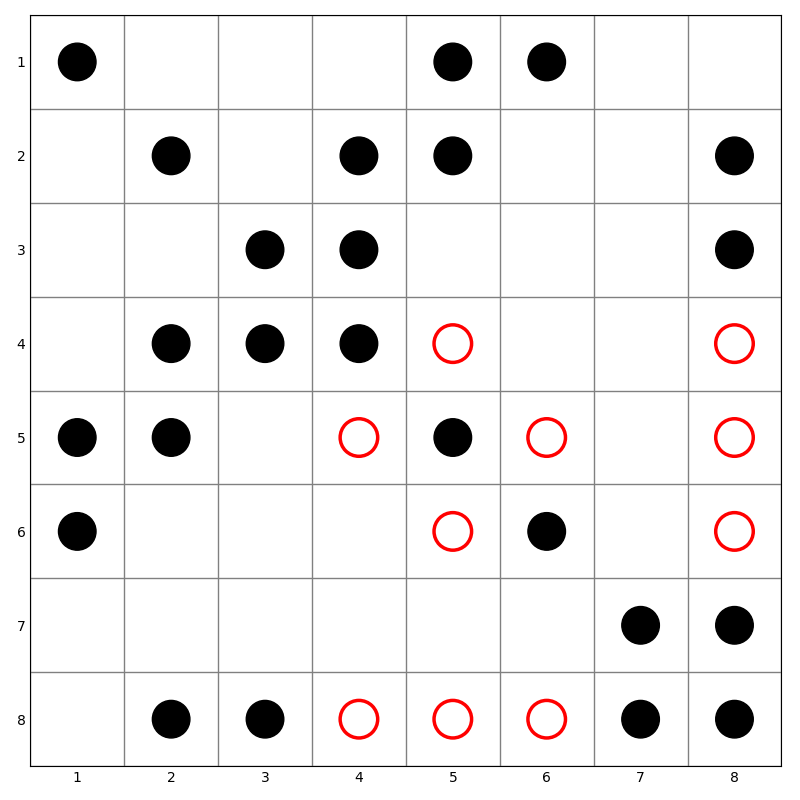
\includegraphics[width=\textwidth]{fig/background/etree-1.png}
        \caption{Sparse matrix structure}
        \label{fig:etree-matrix}
    \end{subfigure}
    \hfill
    \begin{subfigure}[b]{0.45\textwidth}
        \centering
        \vspace{0.5cm}
        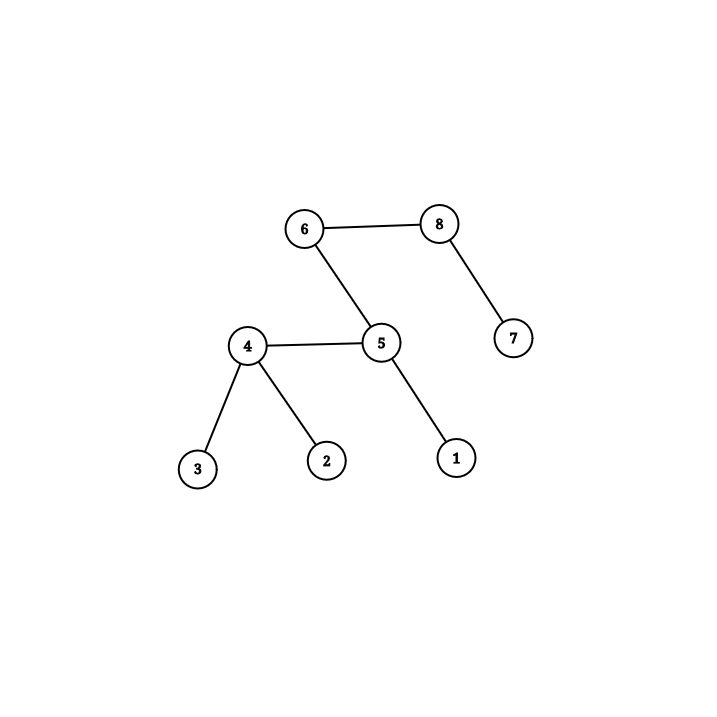
\includegraphics[width=1\textwidth]{fig/background/etree-2.png}
        \caption{Corresponding elimination tree}
        \label{fig:etree-visualization}
    \end{subfigure}
    \caption{Illustration of elimination tree construction for the given sparse symmetric matrix. The sparsity is denoted by filled black circles and the fill-in induced is denoted by hollow red circles.}
    \label{fig:elimination-tree-example}
\end{figure}


\subsection{Symbolic Factorization}

Symbolic factorization determines the sparsity pattern of the Cholesky factor $L$ from the sparsity pattern of matrix $A$ using the elimination tree. It does not involve any numerical computations and relies solely on the structure of the original matrix.

The key insight is that the sparsity structure of each column in $L$ can be computed by analyzing how structural information propagates through the elimination tree. Each column inherits structure from two sources: the original matrix $A$ and the previously computed columns corresponding to its children in the elimination tree.

\begin{definition}[Column Structure Inheritance]
For column $j$ of the Cholesky factor $L$, the nonzero pattern is determined by:
\begin{itemize}
    \item Direct inheritance: All nonzero entries from column $j$ of the original matrix $A$ that lie on or below the diagonal
    \item Indirect inheritance: All entries from the union of nonzero patterns of columns corresponding to children of $j$ in the elimination tree, restricted to rows numbered greater than $j$
\end{itemize}
\end{definition}

This inheritance pattern reflects the computational dependencies during numerical factorization—column $j$ can only be processed after all its children in the elimination tree have been completed.

\begin{algorithm}
\SetKwInOut{Input}{Input}\SetKwInOut{Output}{Output}
\Input{Sparsity pattern of matrix $A$, elimination tree $T(A)$}
\Output{Sparsity pattern of Cholesky factor $L$}
\BlankLine
Initialize $\text{column\_structure}[1 \ldots n]$ as empty sets\;
\For{$j = 1$ \KwTo $n$ \tcp*{in postorder traversal of $T(A)$}}{
    \tcp{Direct inheritance from original matrix}
    $\text{column\_structure}[j] \leftarrow \{i \geq j : A[i,j] \neq 0\}$\;
    \BlankLine
    \tcp{Indirect inheritance from children in elimination tree}
    \ForEach{child $c$ of $j$ in $T(A)$}{
        $\text{column\_structure}[j] \leftarrow \text{column\_structure}[j] \cup \{i \in \text{column\_structure}[c] : i > j\}$\;
    }
    \BlankLine
    \tcp{Record structure for column $j$ of $L$}
    $\text{pattern}(L[:,j]) \leftarrow \text{column\_structure}[j]$\;
}
\Return{$\text{pattern}(L)$}
\caption{Elimination Tree Symbolic Factorization}
\label{alg:symbolic_factorization}
\end{algorithm}

The postorder traversal ensures that each column is processed only after all its descendants in the elimination tree have been completed, respecting the computational dependencies inherent in the factorization process.


\section{Minimum fill-in and NP-completeness}

When performing Cholesky factorization on a sparse symmetric matrix, we want to minimize fill-in - the new nonzero entries that appear during elimination. This translates to a graph theory problem: given a graph representing the matrix's sparsity pattern, find an elimination order that creates the fewest new edges. Yannakakis \cite{yannakakis_computing_1981} proved that this optimization problem is NP-complete, meaning no polynomial-time algorithm can solve it optimally in general (unless P = NP).

The key insight connecting linear algebra to graph theory is that chordal graphs are essential in proving this. A graph is chordal if every cycle of length $\geq 4$ has a chord (an edge connecting non-consecutive vertices). The fundamental theorem states that a graph has perfect elimination (zero fill-in) if and only if it is chordal, and any elimination process on any graph produces a chordal result. Therefore, the minimum fill-in problem becomes: What is the smallest number of edges we must add to make our graph chordal?

The proof uses a three-step reduction to prove NP-completeness. First, we consider bipartite graphs and their special case, chain graphs. A bipartite graph has vertices split into two independent sets $P$ and $Q$, and it is a chain graph when neighborhoods form a nested sequence: $\Gamma(v\sb{1}) \subseteq \Gamma(v\sb{2}) \subseteq \ldots \subseteq \Gamma(v\sb{k})$. The key property is that a bipartite graph is a chain graph if and only if it contains no pair of independent edges.

Second, for any bipartite graph $G = (P, Q, E)$, we construct $C(G)$ by making $P$ into a complete clique (all vertices in $P$ connected), making $Q$ into a complete clique (all vertices in $Q$ connected), and keeping original edges between $P$ and $Q$. The crucial lemma states that $C(G)$ is chordal if and only if $G$ is a chain graph. This works because if $G$ has independent edges, they create a 4-cycle in $C(G)$ with no chord. Conversely, if $G$ is a chain graph, $C(G)$ has a perfect elimination order.

Third, the reduction uses the Optimal Linear Arrangement Problem, which asks: given a graph, arrange vertices on a line to minimize the sum of distances between adjacent vertices. This problem is known to be NP-complete. Yannakakis constructs an transformation where, given graph $G$ with $n$ vertices and $m$ edges, he creates bipartite graph $G'$ where part $P$ has one vertex for each vertex in $G$, and part $Q$ has an elaborate gadget structure with $2m + n^2 - d(v)$ vertices, with connections that encode the linear arrangement constraints. The mathematical relationship is:
\begin{equation}
\text{Minimum fill-in of } G' = \text{Optimal arrangement cost of } G + \frac{n^2(n-1)}{2} - 2m
\end{equation}

This result has practical implications that no perfect algorithm exists, as any algorithm guaranteeing optimal fill-in will require exponential time in the worst case. This explains why practical sparse matrix reordering uses heuristics like minimum degree ordering, nested dissection and such.

\section{Heuristics classification}
\label{sec:heuristics}

There are several heuristics that have been proposed to reduce the fill-in developed over the years. These heuristics can be broadly classified in the following categories: Bandwidth minimization, minimum degree (and it's variants), nested dissection, banded structure methods using hypergraphs, and recently, machine learning approaches. 

\subsection{Bandwidth Minimization}

Bandwidth minimization refers to the problem of permuting the rows and columns of a matrix such that the non-zero entries are as close to the diagonal as possible.  Gaussian elimination can be performed in $O(nb^2)$ time on matrices of dimension $n$ and bandwidth $b$, which is faster than the forward $O(n^3)$ algorithm when $b$ is smaller than $n$ (Lim A. et al., 2006a).  Additionally, this problem is NP-complete, but several heuristics have been developed to approximate the optimal solution.

The Cuthill-McKee algorithm \cite{cuthill_reducing_1969} employs breadth-first search to reduce matrix bandwidth by generating level structures. However, it has computational limitations and may not achieve optimal bandwidth reduction. The Reverse Cuthill-McKee algorithm \cite{george_computer_1981} addresses these issues by reversing the ordering, while the GPS algorithm by Gibbs et al. provides an alternative level structure approach.

We take a look at the reverse Cuthill-McKee algorithm, which is still widely used in practice. 

[write the pseudocode here]

\subsection{Minimum Degree}

The minimum degree algorithm \cite{tinney_direct_1967} determines the order in which to eliminate variables (or pivot) during Gaussian elimination to minimize fill-in (creation of new non-zero entries) in sparse matrices. At each step, it chooses the node with the minimum degree (fewest connections) for elimination.

The minimum degree algorithm operates on the adjacency graph of the sparse matrix. It begins by initializing the graph, where each vertex represents a variable. At each iteration, the algorithm selects the vertex with the smallest degree (i.e., the fewest neighbors), which corresponds to the variable whose elimination is expected to introduce the least fill-in. Upon elimination, the chosen vertex is removed from the graph, and all its neighbors are connected to each other, forming a clique to preserve the matrix structure. The degrees of the affected vertices are then updated to reflect the new connections. This process is repeated until all vertices have been eliminated. The resulting elimination order directly determines the pivot sequence used during matrix factorization.

Variants of the minimum degree algorithm include:

\begin{enumerate}
    \item Multiple Minimum Degree (MMD) \cite{liu_modification_1985}

    When multiple nodes have the same minimum degree, uses additional tie-breaking rules. Often selects based on secondary criteria like external degree or node numbering.

    \item Approximate Minimum Degree (AMD) \cite{amestoy_approximate_1996}

    Uses approximations to avoid expensive exact degree calculations. Employs concepts like "supervariables" and "element absorption". Much faster than exact minimum degree while maintaining similar fill-in quality.

    \item Constrained Minimum Degree

    Incorporates additional constraints (like maintaining bandwidth). Balances minimum degree objective with other structural requirements.

\end{enumerate}

\subsection{Nested Dissection}

Nested dissection is a divide and conquer heuristic for the solution of sparse symmetric systems of linear equations based on graph partitioning. Nested dissection can be viewed as a recursive divide-and-conquer algorithm on an undirected graph; it uses separators in the graph, which are small sets of vertices whose removal divides the graph approximately in half  \cite{lipton_generalized_1979}.

\begin{figure}[htbp]
    \centering
    \begin{subfigure}[b]{0.45\textwidth}
        \centering
        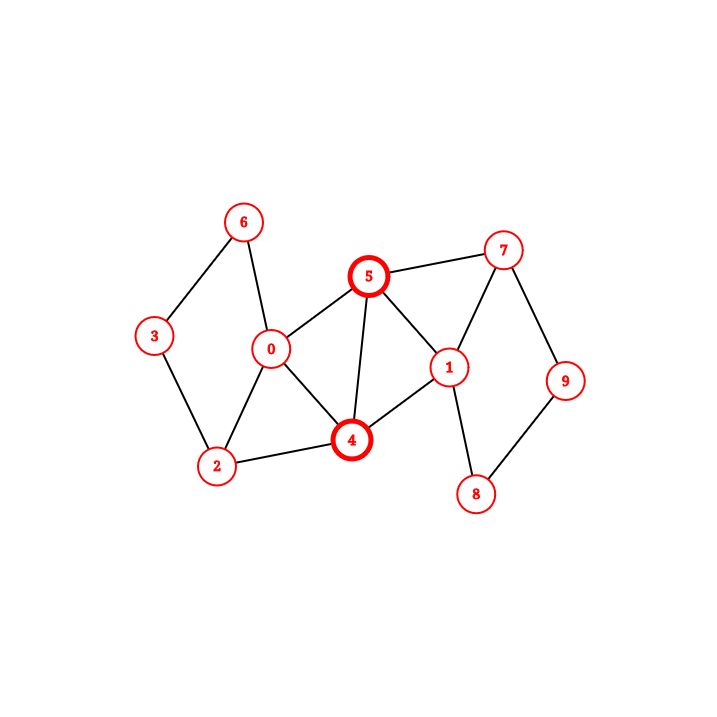
\includegraphics[width=\textwidth]{fig/background/nd-1.png}
        \caption{Original graph before separator identification}
        \label{fig:nd-original}
    \end{subfigure}
    \hfill
    \begin{subfigure}[b]{0.45\textwidth}
        \centering
        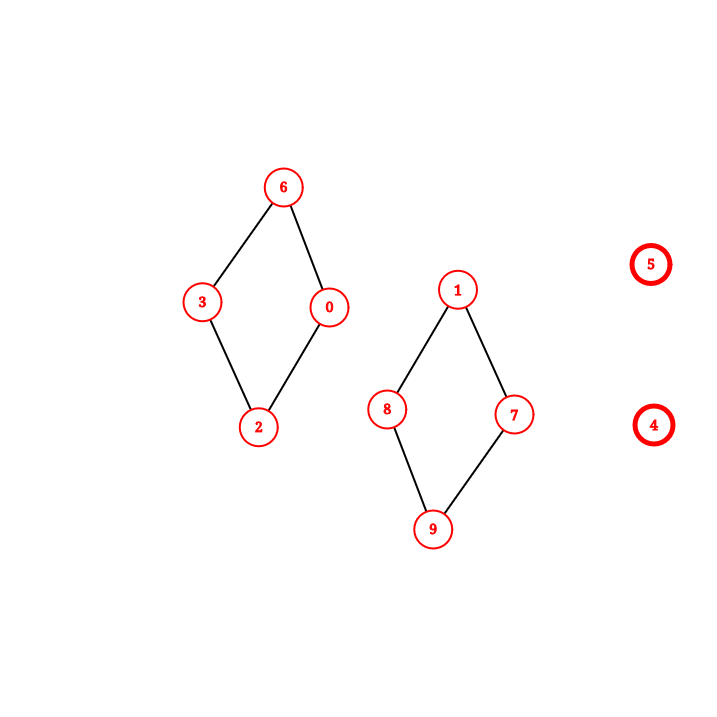
\includegraphics[width=\textwidth]{fig/background/nd-2.png}
        \caption{Graph after separator removal showing partitioned subgraphs}
        \label{fig:nd-separated}
    \end{subfigure}
    \caption{Separator identification process. The separator vertices divide the graph into approximately equal subgraphs}
    \label{fig:nested-dissection}
\end{figure}

Nested dissection consists of the following steps: Form an undirected graph in which the vertices represent rows and columns of the system of linear equations, and an edge represents a nonzero entry in the sparse matrix representing the system. Recursively partition the graph into subgraphs using separators, small subsets of vertices the removal of which allows the graph to be partitioned into subgraphs with at most a constant fraction of the number of vertices. Perform Cholesky decomposition (a variant of Gaussian elimination for symmetric matrices), ordering the elimination of the variables by the recursive structure of the partition: each of the two subgraphs formed by removing the separator is eliminated first, and then the separator vertices are eliminated \cite{george_nested_1973}. 

All the sequential algorithms for determining the elimination ordering of a graph G can be described by the following general algorithm: Generate the tree of separators for G and perform a tree traversal on the separator tree to order the vertices, where this traversal must visit a node before any of its parents.

\subsection{Hypergraph partitioning and other methods}

In recent years, hypergraph partitioning methods \cite{catalyurek_hypergraph_2011} have been proposed to reduce fill-in during sparse matrix factorization. Hypergraphs generalize graphs by allowing edges (hyperedges) to connect more than two vertices, making them well-suited for modeling complex relationships in sparse matrices. In this paper we explore another Hypergraph based reordering method, 

Other methods include machine learning approaches that learn optimal ordering strategies using reinforcement learning. One such approach is Alpha Elimination \cite{dasgupta_alpha_2023} which uses Convolutional Neural Networks (CNNs) and reinforcement learning to predict the next node to eliminate based on the current state of the graph. We have explored a more flexible architecture but fails with scalability, which we discuss in Chapter \ref{ch:other_approaches}.

